\documentclass{scrreprt}
\usepackage[english]{babel}
\usepackage[T1]{fontenc}
\usepackage{lmodern}
\usepackage{blindtext}
\usepackage[utf8]{inputenc}
\usepackage{siunitx} %For unit handling%
\renewcommand{\familydefault}{\sfdefault}
\newcommand{\unit}[1]{\ensuremath{\, \mathrm{#1}}}
\usepackage{amssymb, amsmath, cancel, ulem, graphicx, float, tabularx, multirow, bm}
\usepackage{amsmath}

\setcounter{secnumdepth}{5}
\setcounter{tocdepth}{5}

\author{Urs Gerber\\09-921-156 \and Gian-Luca Mateo\\11-113-545}
\date{7th of March 2013}

\title{Transverse oscillation of a string}
\subtitle{Practical course report}

\begin{document}

\maketitle

\tableofcontents
\newpage

\chapter{Experiment: Transverse oscillation of a string}
\section{Introduction}

\subsection{Goal of the experiment}
The goal of this experiment is to experimentally verify the stationary solutions of the wave equation. In order to do this, we are going to look for resonance frequencies of a string with two fixed ends.
\subsection{Theory}
Throughout the report, you will encounter the following symbols worth explaining:
\begin{itemize}
\item $\mu$ : the longitudinal mass density $[\unit{\frac{kg}{m}}]$
\item $\lambda$: The wavelength $[\unit{m}]$
\item $\omega$: The oscillating frequency $[\unit{Hz}]$
\item $A$: The amplitude $[\unit{m}]$
\item $L$: The length of the string $[\unit{m}]$
\item $v$: The transverse propagation speed $\unit{[\frac{m}{s}}]$
\end{itemize}

\paragraph*{Task 4}
The total energy $E$ of the oscillating string in ground state $n=1$ is:
\begin{equation}
E=\frac{1}{4} \mu \lambda \omega^2 A^2
\end{equation}
Proof:

\begin{align}
E &= E_{\text{kin}} + E_{\text{pot}}\\
E_{\text{kin}} &= \frac{1}{2} m v^2 , \quad E_{\text{pot}} = \frac{k}{2} x^2\\
x(t) &= A \sin{\omega t} , \quad v(t) = \frac{dx}{dt} = \dot{x}(t) = A \omega \cos{\omega t}\\
\Rightarrow E &= \frac{k}{2} A^s \sin^2{\omega t} + \frac{1}{2} m A^2 \omega^2 \cos{\omega t}
\end{align}

Using

\begin{equation}
\bar{E} = \frac{1}{T} \int_0^T{E(t') dt}
\end{equation}

we find:
\begin{align}
\bar{E} &= \frac{1}{T} \int_0^T{\frac{k}{2} A^2 \sin^2{\omega t} + \frac{1}{2} m A^2 \omega^2 \cos{\omega t}}\,dt\\
\stackrel{k=m\omega^2}{=}& \frac{1}{T} \int_0^T{\frac{1}{2} A^2 m \omega^2 \sin^2{\omega t} + \frac{1}{2} m A^2 \omega^2 \cos{\omega t}} \,dt\\
&= \frac{1}{T}\int_0^T{\frac{1}{2} m A^2 \omega^2 \underbrace{(\sin^2{\omega t}+\cos^2{\omega t})}_{1} } \,dt\\
& = \frac{1}{T}\int_0^T \! \frac{1}{2}mA^2\omega^2 \, dt\\
& =\frac{1}{2}mA^2\omega^2\\
l &= \frac{\lambda}{2} \Rightarrow m = \mu l = \frac{\mu \lambda}{2}\\ 
\Rightarrow \bar{E} &= \frac{1}{4}\mu \lambda A^2\omega^2
\end{align}

\subsection{Error estimation and calculation}
We found the spring balance's measurements to be the most problematic. The marks on the balance were too bold and fuzzy to be read accurately. This inaccuracy is even enlarged by the fact that the scale was using Kiloponds as a unit of measurement. We estimated the force reading to be within $\pm 0.2\unit{kp} = \pm 1.96 \unit{N}$ (see Experiment setup and execution).\\

\begin{equation}
v = \sqrt{\frac{K}{\mu}} = \lambda_n f_n \Rightarrow f_n = \frac{1}{\lambda} \sqrt{\frac{K}{\mu}} 
\end{equation}

\begin{equation} \label{eq:relerror}
\Rightarrow \frac{s_{\bar{f}}}{\bar{f}} = \frac{1}{2} \frac{s_{\overline{K}}}{\overline{K}}
\end{equation}

\section{Experiment setup and execution}
The Materials for this experiment are the following: 
\subsection{Materials used}
\begin{itemize}
  \item A string and a clamping mechanism which allows adjusting and measuring the force applied to the string using a string balance. The spring balance was rated 5 $\unit{kp} = 49.03\unit{N}$ maximum.
  \item Two clamps with connectors for standard electic wires.
  \item A wave-generator (Model Ultron SRG-24, adjustable output frequency of 1-100 Hz with a selectable multiplier x1, x10, x100 and x1k, yielding an effective RF range of 0-100 KHz)
  \item An AC amplifier (Custom built, rated 20V input voltage and 2$\Omega$ output impedance)
  \item A multimeter (Model FLUKE 175 True RMS Multimeter)
  \item A magnet
  \item 6 wires
\end{itemize}

\subsection{Assembly}

\begin{figure}[H]
\center
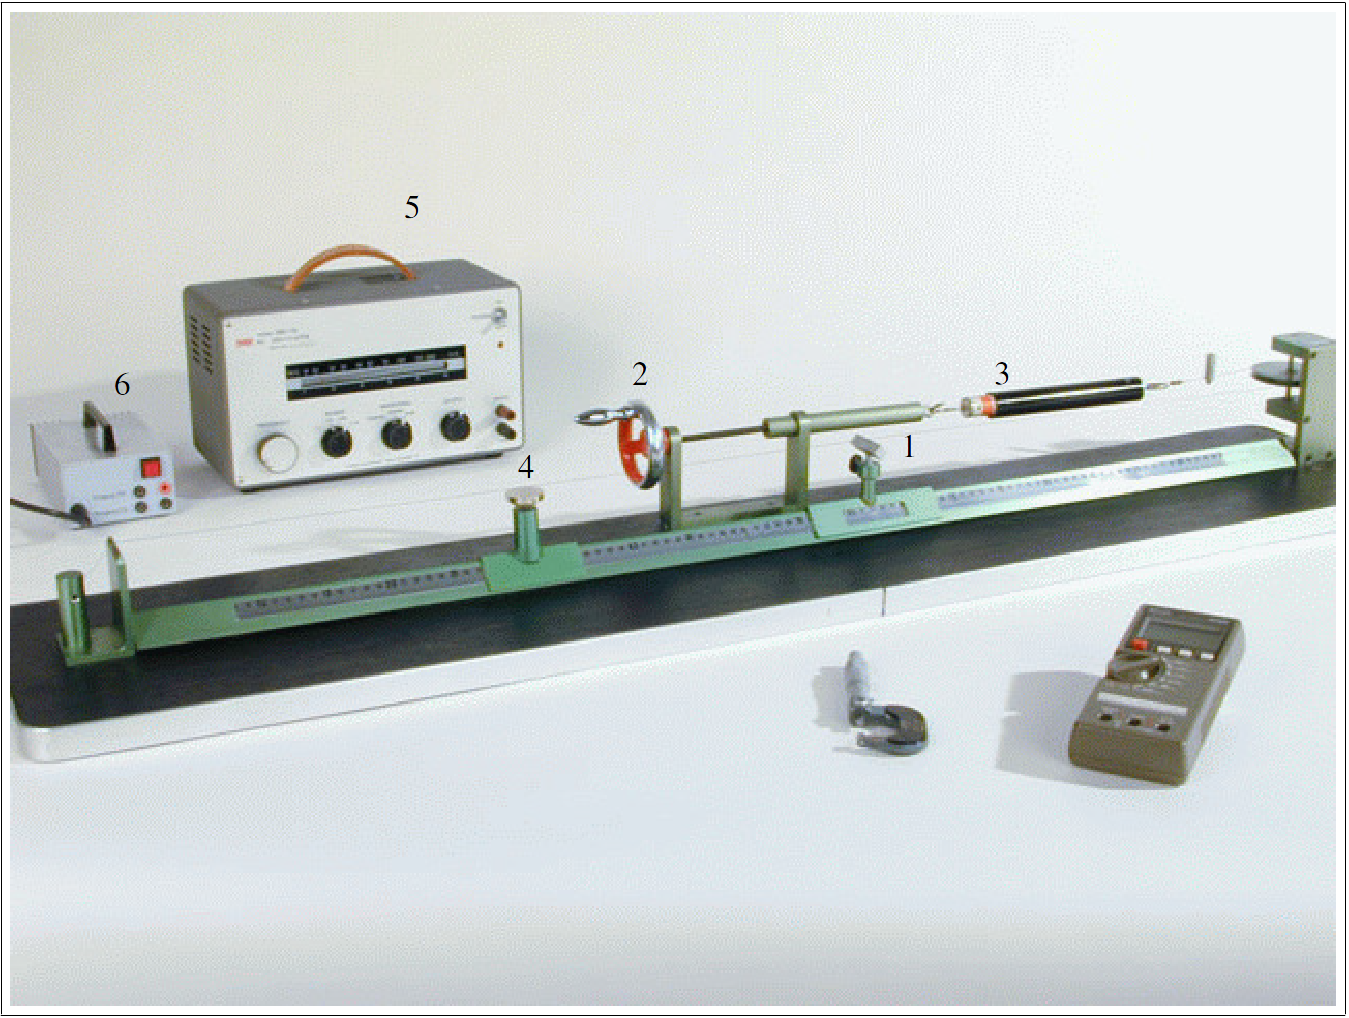
\includegraphics[width=0.9\textwidth]{img/WaveSetup.PNG}
\caption{Experiment assembly}
\end{figure}

The string is fitted in the clamping mechanism and the clamps are fixed on either side of the fixed string. The magnet is then fitted underneath the string, allowing it to be moved along the string. Next, the electric equipment is installed by connecting the outputs of the wave generator (5) parallel to both the inputs of the amplifier (6) and the multimeter. The clamps are then connected to the outputs of the amplifier.
To avoid putting too much strain on the amplifier, we set the output voltage to just shy of $2\unit{V}$.\\
Due to the Lorentz force the electrons moving through the wire will experience a force when travelling through the magnet's magnetic field and consequently the wire will be pushed sideways alternatingly, producing an oscillation. Once a stationary mode is reached, two opposed harmonic waves will create a standing wave, which was made audible by a resonance chamber attached to the string assembly.\\
The adjustable string length was set to exactly 1 Meter, simplifying calculations. We chose tensile forces of $K_1=(1.5 \pm 0.2) \unit{kp} =(14.7 \pm 1.96)\unit{N}$ and $K_2=(3.0 \pm 0.2) \unit{kp} =(29.4 \pm 1.96) \unit{N}$ at a later time.\\
Using the frequency regulator on the wave-generator, we now proceed to searching the spectrum for resonances, listening and looking closely at the string.

\section{Measurements and Analysis}

\subsection[Frequency]{Frequency $\bm{f}$}

\begin{table}[H]
	\center
	\begin{tabular}{|c|c|cccccc|}
	\cline{2-8}
	 \multicolumn{1}{c|}{}& $n=$ & 1 & 2 & 3 & 4 & 5 & 6\\  \hline
	\multirow{2}{*}{$l=1\unit{m}$} & $K_1=14.7\unit{N}$ & 63.8 & 125.1 & 186.9 & 248.4 & 311.0 & 371.6\\
	& $K_2=29.4\unit{N}$ & 87.23 & 172.0 & 258.5 & 344.0 & 430.4 & 514.6\\
	\hline
	\end{tabular}
	\caption{String frequency $f$ in Hertz [Hz] at highest oscillation amplitude under distinct tensile forces $F_1, F_2$ and in oscillation modes $n=1,...,6$ with string length $l=1\unit{m}$}
\end{table}

\subsection[Mass per length]{Mass per length $\bm{\mu}$}

\begin{equation}
v=\sqrt{\frac{K}{\mu}}=\lambda_n f_n \Rightarrow \mu = \frac{K}{\lambda_n^2 f_n^2} 
\end{equation}

\begin{table}[H]
	\center
	\begin{tabular}{|c|c|cccccc|}
	\cline{2-8}
	 \multicolumn{1}{c|}{}& $n=$ & 1 & 2 & 3 & 4 & 5 & 6\\  \hline
	\multirow{2}{*}{$l=1\unit{m}$} & $K_1$ & 9.029e-4 & 9.393e-4 & 9.469e-4 & 9.530e-4 & 9.499e-4 & 9.581e-4\\
	& $K_2$ & 9.660e-4 & 9.938e-4 & 9.899e-4 & 9.938e-4 & 9.919e-4 & 9.992e-4\\
	\hline
	\end{tabular}
	\caption{Calculated mass per length $\mu$ in [$\frac{\unit{kg}}{\unit{m}}$]}
\end{table}

\begin{table}[H]
\center
\begin{tabular}{|c|ccc|}
\cline{2-4}
\multicolumn{1}{c|}{}& $\bar{\mu}$ & $s_{\mu}$ & $s_{\bar{\mu}}$\\ \hline
$F_1$ & 9.417e-4 & 2.002e-5 & 8.954e-6 \\ \hline
$F_2$ & 9.891e-4 & 1.175e-5 & 5.255e-6\\ \hline
\end{tabular}
\caption{Mean $\bar{\mu}$, standard deviation $s_{\mu}$ and standard error of mean $s_{\bar{\mu}}$} of mass per length $\mu$ in [$\unit{\frac{kg}{m}}$]
\end{table}

\subsection[Transervse propagation speed]{Transverse propagation speed $\bm{v}$}

\begin{equation}
v=\lambda_n f_n
\end{equation}

\begin{table}[H]
	\center
	\begin{tabular}{|c|c|cccccc|}
	\cline{2-8}
	 \multicolumn{1}{c|}{}& $n=$ & 1 & 2 & 3 & 4 & 5 & 6\\  \hline
	\multirow{2}{*}{$l=1\unit{m}$} & $K_1$ & 127.6 & 125.1 & 124.6 & 124.2 & 124.4 & 123.867\\
	& $K_2$ & 174.46 & 172.0 & 172.333 & 172.0 & 172.16 & 171.533\\
	\hline
	\end{tabular}
	\caption{Calculated transverse propagation speed $v$ in [$\unit{\frac{m}{s}}]$}
\end{table}

\begin{table}[H]
\center
\begin{tabular}{|c|ccc|}
\cline{2-4}
\multicolumn{1}{c|}{}& $\bar{v}$ & $s_{v}$ & $s_{\bar{v}}$\\ \hline
$K_1$ & 124.961 & 1.357 & 0.607 \\ \hline
$K_2$ & 172.414 & 1.037 & 0.464\\ \hline
\end{tabular}
\caption{Mean $\bar{v}$, standard deviation $s_{v}$ and standard error of mean $s_{\bar{v}}$ of transverse propagation speed $v$ in [$\unit{\frac{m}{s}}$]}
\end{table}

\begin{figure}[H]
\center
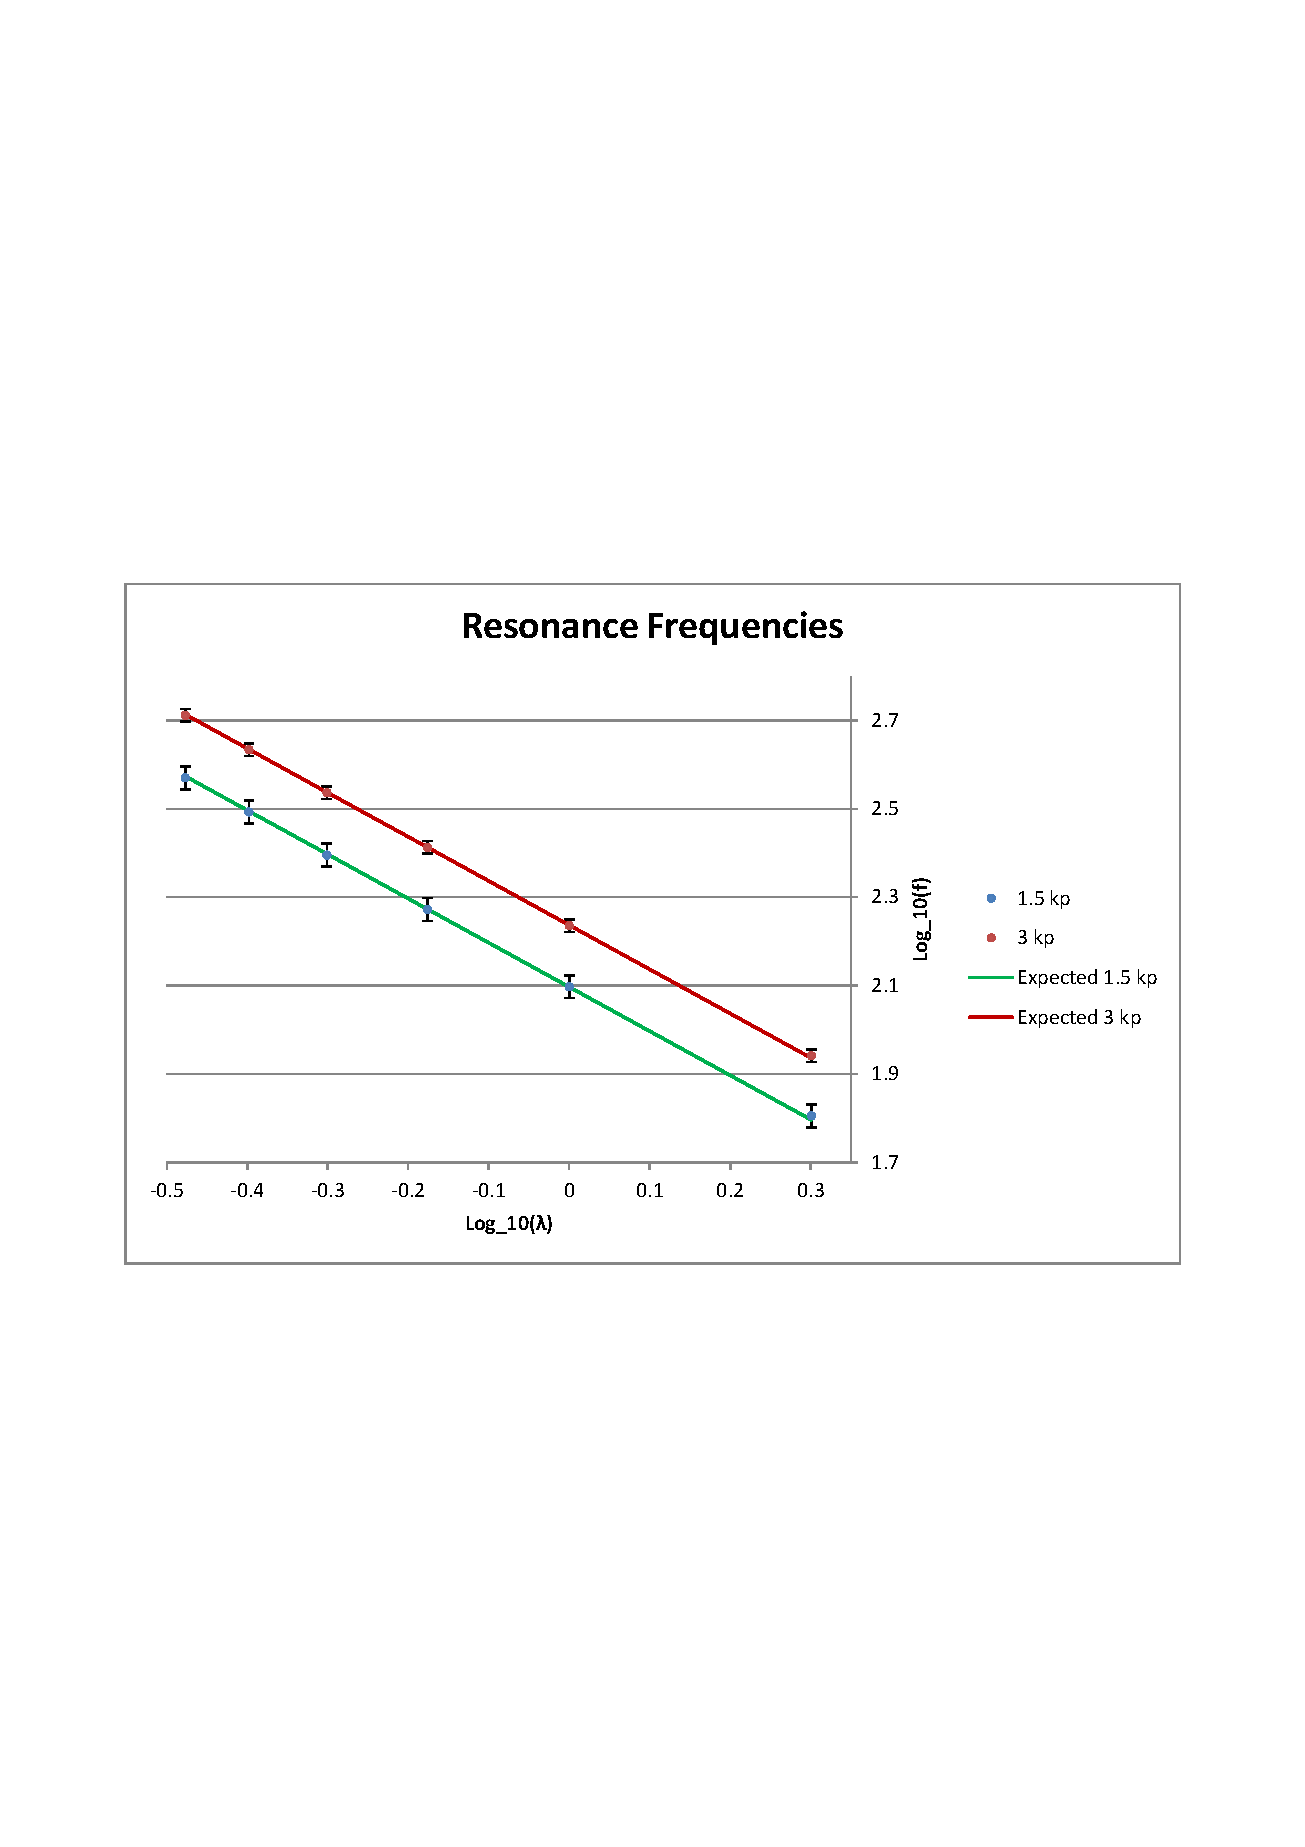
\includegraphics[width=1.0\textwidth]{img/ResonanceFrequencies.pdf}
\caption{Experiment analysis}
\end{figure}

The formula for the expected values is obtained as follows:
\begin{align}
\mu &= \frac{K}{\lambda^2 \cdot f^2}\\
f^2 &= \frac{K}{\lambda^2\cdot\mu}\\
f &= \frac{1}{\lambda}\cdot\sqrt{\frac{K}{\mu}}\\
log(f) &= log\left(\frac{1}{\lambda}\cdot\sqrt{\frac{K}{\mu}}\right)\\
&=log\left(\frac{1}{\lambda}\right) + log\frac{K}{\mu}\\
&=\left(log(1) - log(\lambda)\right) + log\frac{K}{\mu}\\
\Rightarrow log(f) &=-log(\lambda) + log\frac{K}{\mu}
\end{align}

\paragraph*{Error bar calculation} In order to calculate the error bars we used equation \ref{eq:relerror} and the estimated error for the string's tensile force $s_{\overline{K}}=0.2 \unit{kp} = 1.96 \unit{N}$:

\begin{table}[H]
\center
\begin{tabular}{|c|cc|}
\cline{2-3}
\multicolumn{1}{c|}{}& \tiny $\frac{s_{\overline{K}}}{\overline{K}}$ & \tiny$\frac{s_{\bar{f}}}{\bar{f}}$\\ \hline
$K_1$ & \small$\frac{2}{15}$ & \small$\frac{1}{15}$ \\ \hline
$K_2$ & \small$\frac{1}{15}$ & \small$\frac{1}{30}$\\ \hline
\end{tabular}
\caption{Error bar calculation}
\end{table}


\section{Discussion}

\begin{thebibliography}{9}

\bibitem{physcript13}
  Peter Wurz,
  \emph{Anleitung zum Physikpraktikum}
  FS2013

\end{thebibliography}

\end{document}
